%% bare_conf.tex
%% V1.4b
%% 2015/08/26
%% by Michael Shell
%% See:
%% http://www.michaelshell.org/
%% for current contact information.
%%
%% This is a skeleton file demonstrating the use of IEEEtran.cls
%% (requires IEEEtran.cls version 1.8b or later) with an IEEE
%% conference paper.
%%
%% Support sites:
%% http://www.michaelshell.org/tex/ieeetran/
%% http://www.ctan.org/pkg/ieeetran
%% and
%% http://www.ieee.org/

%%*************************************************************************
%% Legal Notice:
%% This code is offered as-is without any warranty either expressed or
%% implied; without even the implied warranty of MERCHANTABILITY or
%% FITNESS FOR A PARTICULAR PURPOSE! 
%% User assumes all risk.
%% In no event shall the IEEE or any contributor to this code be liable for
%% any damages or losses, including, but not limited to, incidental,
%% consequential, or any other damages, resulting from the use or misuse
%% of any information contained here.
%%
%% All comments are the opinions of their respective authors and are not
%% necessarily endorsed by the IEEE.
%%
%% This work is distributed under the LaTeX Project Public License (LPPL)
%% ( http://www.latex-project.org/ ) version 1.3, and may be freely used,
%% distributed and modified. A copy of the LPPL, version 1.3, is included
%% in the base LaTeX documentation of all distributions of LaTeX released
%% 2003/12/01 or later.
%% Retain all contribution notices and credits.
%% ** Modified files should be clearly indicated as such, including  **
%% ** renaming them and changing author support contact information. **
%%*************************************************************************


% *** Authors should verify (and, if needed, correct) their LaTeX system  ***
% *** with the testflow diagnostic prior to trusting their LaTeX platform ***
% *** with production work. The IEEE's font choices and paper sizes can   ***
% *** trigger bugs that do not appear when using other class files.       ***                          ***
% The testflow support page is at:
% http://www.michaelshell.org/tex/testflow/

\documentclass[hidelinks,english,conference]{IEEEtran}

\usepackage{graphicx}
\usepackage{grffile}
\usepackage[T1]{fontenc}
\usepackage{babel}
\usepackage{wrapfig}
\usepackage{hyperref}

\date{\today}


% *** MATH PACKAGES ***
\usepackage{amssymb}
\usepackage{amsmath}

\usepackage{algorithm2e}

\hyphenation{op-tical net-works semi-conduc-tor}

\graphicspath{{Pictures/}}
\begin{document}
\title{Particle Swarm Optimization: Intelligent Parameter Tuning}
\author{\IEEEauthorblockN{Armand Maree}
\IEEEauthorblockA{Department of Computer Science\\
University of Pretoria\\}}
\maketitle

\begin{abstract}
Particle Swarm Optimization (PSO) is a optimization algorithm that models the flocking behaviour of certain species of animals in order to solve stochastic real-value problems. These algorithms use control parameters to make slight adjustments to how the swarm behaves. In this report the author will be discussing the results of using a brute force approach to find these control parameters.
\end{abstract}

\IEEEpeerreviewmaketitle

\section{Introduction}\label{intoductionSection}
A Particle Swarm Optimisor (PSO) is, as described by Lazincia \cite{lazinica2009particle}, an optimization algorithm that attempts to emulate the flocking/schooling behaviour of birds or fish when searching for food. This optimization can occur in a number of dimensions, each spanning across $\mathbb{R}$ \cite{kennedy1997discrete}. Each particle in the swarm has two primary components of influence: cognative and social. A third component, called the inertia weight, is used to regulate the maximum velocity that a particle can move at in a certain direction \cite{eberhart2000comparing}. In this report, the author will explore the feasibility of finding the optimum value for each of these components by using a brute force search in a subset.

\section{Background}
As discussed in section \ref{intoductionSection}, the two components that influence a particle's behaviour is cognative and social. The cognative component refers to the influence that a particle experiences due to the best position it has found so far \cite{shi1998modified}. A more animalistic analogy of this would be that if you feed a bird it will be more inclined to visit your house in the future to get more food. The social component refers to how a particle is influenced by the best position found by other particles in the neighbourhood \cite{shi1998modified}. The analogy here would be that if you feed one bird the other birds in the flock might be more inclined to also visit your house to get food. There is a trade-off between these two components. The cognative component favours exploration of the search space, while the social component favours exploitation of the global best position.

The last parameter is the inertia weight developed by Shi and Eberhart (1998). The role of this parameter is to balance global search and local search. \cite{shi1998modified} and thus controls the velocity a particle can move at. The inertia weight was originally proposed in order to avoid the velocity clamping mechanism that was used before.

In order to test the feasibility of the brute force approach four objective functions were used. 
\begin{itemize}
	\item Spherical
		\begin{equation}\label{sphericalEquation}
			f(\textbf{x})=\sum_{i=1}^{d}x_{i}^{2}
		\end{equation}
	\item Ackley\\ 
		\begin{equation}\label{ackleyEquation}
			f(\textbf{x})=-20e^{\sqrt[-0.2]{\frac{1}{d}\sum_{i=1}^{d}x_{i}^{2}}}-e^{\frac{1}{d}\sum_{i=1}^{d}\cos(2\pi x_{i})}+20+e
		\end{equation}
	\item Michalewicz\\
		\begin{equation}\label{michalewiczEquation}
			f(\textbf{x})=-\sum_{i=1}^{d}[\sin(x_i)\sin^{2*10}(\frac{ix_{i}^{2}}{\pi})]
		\end{equation}
	\item Katsuura\\
		\begin{equation}\label{katsuuraEquation}
			\begin{split}
			f(\textbf{x})=\frac{10}{d^{2}\prod_{i=1}^{d}}(1+i\sum_{j=1}^{32}\frac{\left|2^{j}x_{i}-round(2^{j}x_{i})\right|}{2^{j}})^{\frac{10}{d^{1.2}}}\\-\frac{10}{d^{2}}
			\end{split}
		\end{equation}
\end{itemize}

The topology that was used is the star topology, as prescribed by the project specifications. This model states that all the particles in the swarm are connected to all other particles in the swarm. This means that there is only one neighbourbood and all particles belong to it. This approach means that the global best position (gbest) will be used as the current optimum.

The brute force approach used in this report refers to the systematic exhaustive evaluation of a parameter that falls in a finite set of numbers. Since the range that these three parameters usually fall in is known and small, it might prove to be a feasible option to find these parameters via this approach.

\section{Implementation}
A swarm of 20 particles was used to solve all the objective functions in a 20-dimensional space. The restrictions on $w$, $c_1$ and $c_2$ was specified as follows:
\begin{itemize}
	\item $w \in \left[-1.1, 1.1\right]$
	\item $c_1 + c_2 \in \left(0.0, 5.0\right]$
	\item $c_1 = c_2$
\end{itemize}

Each of these values had a step size of $0.1$.

The velocity, $\textbf{v}_i$, of a particle, $par_i$, will be used to update the position, $\textbf{x}_i$, of $par_i$, as follows:\\
\begin{equation}
	\textbf{x}_i(t+1)=\textbf{x}_i(t) + \textbf{v}_i(t+1)
\end{equation}
where,
\begin{align}\label{velocityEquation}
\begin{split}
	\textbf{v}_i(t+1)=w\textbf{v}_i(t) + c_1\textbf{r}_1 \otimes (\textbf{p}_i(t) - \textbf{x}_i(t)) +\\c_2\textbf{r}_2 \otimes (\textbf{g}_i(t) - \textbf{x}_i(t))
\end{split}
\end{align}
where,\\
\begin{center}
	$\textbf{p}_i$ refers to the personal best position of $par_i$,\\
	and,\\
	$\textbf{g}_i$ refers to the global best position of the entire swarm.
\end{center}

$\otimes$ refers to componentwise multiplication of vectors.\\
$w$ used in equation \ref{velocityEquation} is the inertia weight as discussed in section \ref{intoductionSection}.\\
$c_{1}$ and $c_{2}$  used in equation \ref{velocityEquation} represents the cognative and social components respectively as discussed in section \ref{intoductionSection}.

Since PSO is a stochastic algorithm a single run can have abnormally good or bad results. Each set of possible combinations between $w$, $c_{1}$ and $c_{2}$ has been tested 30 times and the average result of all 30 runs has been taken as the optimal result for the specific configuration. The best configuration's result, along with the corresponding values for $w$, $c_{1}$ and $c_{2}$ is stored each time a new optimum is found.

A simple pseudo code version of the entire algorithm is shown in algorithm \ref{SolvePSO} and \ref{parameterFindAlgo}:
\begin{algorithm}
\SetAlgoLined
\caption{Main PSO Algorithm}\label{SolvePSO}initializeSwarm()\\
\While{not (stopping condition)}{
	\ForEach{particle in swarm}{
		var objectiveFunctionResult = particle.getObjectiveFunctionResult()
		\If{objectiveFunctionResult < particle.personalBest}{
			/* Save current position as personal best */
		}
		\If{objectiveFunctionResult < particle.neighbourhoodBest}{
			/* Save current position as neighbourhood best */
		}
	}
	\ForEach{particle in swarm}{
		particle.updateVelocity()
		particle.updatePosition()
	}
}
return particle[0].neighbourhoodBest
\end{algorithm}

\begin{algorithm}
\SetAlgoLined
\caption{PSO Parameter Finding}\label{parameterFindAlgo}
var bestSolution = infinity
\For{w <- -1.1 to 1.1}{
	\For{c1 <- 0.1 to 2.5}{
		c2 = c1\\
		\For{currentRun <- 1 to 30}{
			/* call "solvePSO" function which is algorithm \ref{SolvePSO} */\\
			var bestResult += objectiveFunction(solvePSO())
		}
		\If{bestResult/30 < bestSolution["result"]}{
			bestSolution["result"] = bestResult\\
			bestSolution["w"] = w\\
			bestSolution["c1"] = c1\\
			bestSolution["c2"] = c2
		}
	}
}
\end{algorithm}


\section{Research Results}\label{researchResultsSection}
The algorithm managed to obtain values for all the parameters to all the objective functions. The results were as follows:
\begin{itemize}
	\item Spherical\\
		\begin{itemize}
			\item $Optimum \approx 0.0$
			\item Variance across 30 runs $ \approx 0.0$
			\item $w = 0.6$
			\item $c1 = 0.6$
			\item $c2 = 0.6$
			\item $x_{0} \approx 0.0$
			\item $x_{1} \approx 0.0$
			\item $x_{2} \approx 0.0$
			\item $x_{3} \approx 0.0$
			\item $x_{4} \approx 0.0$
			\item $x_{5} \approx 0.0$
			\item $x_{6} \approx 0.0$
			\item $x_{7} \approx 0.0$
			\item $x_{8} \approx 0.0$
			\item $x_{9} \approx 0.0$
			\item $x_{10} \approx 0.0$
			\item $x_{11} \approx 0.0$
			\item $x_{12} \approx 0.0$
			\item $x_{13} \approx 0.0$
			\item $x_{14} \approx 0.0$
			\item $x_{15} \approx 0.0$
			\item $x_{16} \approx 0.0$
			\item $x_{17} \approx 0.0$
			\item $x_{18} \approx 0.0$
			\item $x_{19} \approx 0.0$
			
		\end{itemize}
	\item Ackley\\
		\begin{itemize}
			\item $Optimum \approx 0.0$
			\item Variance across 30 runs $ \approx 0.0$
			\item $w = 0.6$
			\item $c1 = 0.6$
			\item $c2 = 0.6$
			\item $x_{0} \approx 0.0$
			\item $x_{1} \approx 0.0$
			\item $x_{2} \approx 0.0$
			\item $x_{3} \approx 0.0$
			\item $x_{4} \approx 0.0$
			\item $x_{5} \approx 0.0$
			\item $x_{6} \approx 0.0$
			\item $x_{7} \approx 0.0$
			\item $x_{8} \approx 0.0$
			\item $x_{9} \approx 0.0$
			\item $x_{10} \approx 0.0$
			\item $x_{11} \approx 0.0$
			\item $x_{12} \approx 0.0$
			\item $x_{13} \approx 0.0$
			\item $x_{14} \approx 0.0$
			\item $x_{15} \approx 0.0$
			\item $x_{16} \approx 0.0$
			\item $x_{17} \approx 0.0$
			\item $x_{18} \approx 0.0$
			\item $x_{19} \approx 0.0$
		\end{itemize}
	\item Michalewicz\\
		\begin{itemize}
			\item $Optimum \approx -19.786$
			\item Variance across 30 runs $ \approx 0.0$
			\item $w = 0.6$
			\item $c1 = 0.6$
			\item $c2 = 0.6$
			\item $x_{0} \approx 623.61$
			\item $x_{1} \approx 1.57$
			\item $x_{2} \approx 1.28$
			\item $x_{3} \approx 1.92$
			\item $x_{4} \approx 1.72$
			\item $x_{5} \approx 1.57$
			\item $x_{6} \approx 7.83$
			\item $x_{7} \approx 1.76$
			\item $x_{8} \approx 1.28$
			\item $x_{9} \approx 1.57$
			\item $x_{10} \approx 1.5$
			\item $x_{11} \approx 1.43$
			\item $x_{12} \approx 1.63$
			\item $x_{13} \approx 1.57$
			\item $x_{14} \approx 1.52$
			\item $x_{15} \approx 1.67$
			\item $x_{16} \approx 1.62$
			\item $x_{17} \approx 1.39$
			\item $x_{18} \approx 1.53$
			\item $x_{19} \approx 1.49$
		\end{itemize}
	\item Katsuura\\
		\begin{itemize}
			\item $Optimum \approx 0.04$
			\item $w = 0.6$
			\item $c1 = 0.6$
			\item $c2 = 0.6$
			\item $x_{0} \approx -1.0 \times 10^{4}$
			\item $x_{1} \approx -1.5 \times 10^{6}$
			\item $x_{2} \approx 2.1 \times 10^{6}$
			\item $x_{3} \approx -1.8 \times 10^{4}$
			\item $x_{4} \approx 1.6 \times 10^{6}$
			\item $x_{5} \approx -2.1 \times 10^{6}$
			\item $x_{6} \approx 3.2 \times 10^{5}$
			\item $x_{7} \approx 1.8 \times 10^{6}$
			\item $x_{8} \approx 1.0 \times 10^{7}$
			\item $x_{9} \approx 1.3 \times 10^{6}$
			\item $x_{10} \approx 2.6 \times 10^{6}$
			\item $x_{11} \approx 5.2 \times 10^{5}$
			\item $x_{12} \approx -1.8 \times 10^{5}$
			\item $x_{13} \approx -3.3 \times 10^{4}$
			\item $x_{14} \approx -3.0 \times 10^{6}$
			\item $x_{15} \approx 1.9 \times 10^{4}$
			\item $x_{16} \approx 1.7 \times 10^{4}$
			\item $x_{17} \approx 5.7 \times 10^{5}$
			\item $x_{18} \approx 4.8 \times 10^{5}$
			\item $x_{19} \approx 5.2 \times 10^{6}$
		\end{itemize}
\end{itemize}

\section{Conclusion}
As expected, the results in section \ref{researchResultsSection} indicate, if a small range for each of the three parameters is known, it is possible to find the optimum value for an objective function. This can even be done is a fairly short amount of time if the objective function is simple, as is the case with equation \ref{sphericalEquation}, \ref{ackleyEquation} and \ref{michalewiczEquation}, but as the complexity (or rather computational time) grows, like with equation \ref{katsuuraEquation}, this process can become quite lengthy.

Thus, if an equation does not contain a large amount of computational demanding steps, this brute force approach might be a feasible option since it is simple and quick to implement.


\bibliographystyle{unsrt}
\bibliography{bibliography}

\section*{Appendix}
Here follows some screenshots of the results outlined in section \ref{researchResultsSection}.
\begin{figure}[!h]\centering
	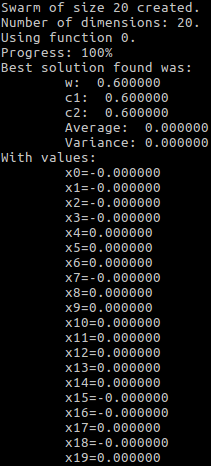
\includegraphics[width=4.5cm]{spherical_results.png}
	\caption{Spherical Objective Function Results}
\end{figure}
\begin{figure}[!h]\centering
	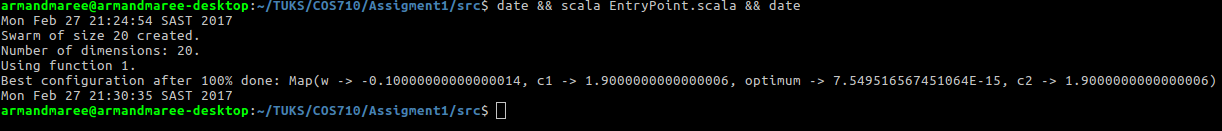
\includegraphics[width=4.5cm]{ackley_results.png}
	\caption{Ackley Objective Function Results}
\end{figure}
\begin{figure}[!h]\centering
	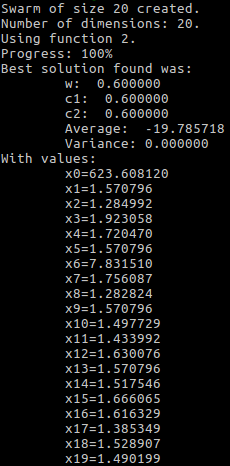
\includegraphics[width=4.5cm]{michalewicz_results.png}
	\caption{Michalewicz Objective Function Results}
\end{figure}
\begin{figure}[!h]\centering
	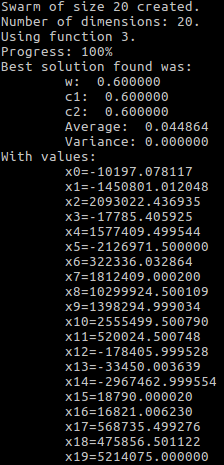
\includegraphics[width=4.5cm]{katsuura_results.png}
	\caption{Katsuura Objective Function Results}
\end{figure}

\end{document}


